%
% Permission is granted to copy, distribute and/or modify this
% document under the terms of the Creative Common by-nc-sa License
% version 3.0 (CC BY-NC-SA 3.0). A copy of the license can be found at
% http://creativecommons.org/licenses/by-nc-sa/3.0/legalcode.
%

\usepackage[french]{babel}
\usepackage{tikz}
\usetikzlibrary{shapes}
\usetikzlibrary{positioning}
\usepackage{color}
\usepackage{amsmath, amsthm, amscd, amssymb, amsfonts, amsxtra}
\usepackage{stmaryrd}
\usepackage{graphicx, wrapfig, lipsum}

\tikzset{
  every overlay node/.style={
    %draw=black,fill=white,rounded corners,
    anchor=north west, inner sep=0pt,
  },
}
% Usage:
% \tikzoverlay at (-1cm,-5cm) {content};
% or
% \tikzoverlay[text width=5cm] at (-1cm,-5cm) {content};
\def\tikzoverlay{
   \tikz[remember picture, overlay]\node[every overlay node]
}

% Highlight macros
\newcommand{\highlight}[1]{\textcolor{structure.fg}{\bfseries #1}}

%% Title, subtitle, authors, institute, date, ...
\title{Implémentation de fonctions en éponge}

\author[Amélie Guémon \& Ida Tucker]{Amélie Guémon\\Ida Tucker\\[.25em]
\texttt{\scriptsize <amelie.guemon@etu.u-bordeaux.fr>}\\[-.25em]
\texttt{\scriptsize <ida.tucker@etu.u-bordeaux.fr>}\\}

\institute[Master CSI]{Master CSI, Université de Bordeaux, France}

\date{\today}

%%%%%%%%%%%%%%%%%%%%%%%%%%[ Document ]%%%%%%%%%%%%%%%%%%%%%%%%%%
\begin{document}

\begin{frame}
  \vspace{3.5em}
  \titlepage

  \begin{center}
    
\includegraphics[scale=.2]{cc-by-nc-sa.pdf}
  \end{center}
\end{frame}

\begin{frame}
  \frametitle{Plan}
  \tableofcontents[subsectionstyle=hide]
\end{frame}

%%%%%%%%%%%%%%%%%%%%%%%%%%%%[ Introduction ]%%%%%%%%%%%%%%%%%%%%%%%%%%

\begin{frame}[fragile]
  \frametitle{Définition: fonction de hashage}
  \vfill

Une fonction de hashage est une application qui associe à un ensemble de départ infini $\{0,1\}^*$ un ensemble d'arrivée fini  $\{0,1\}^n$ constitué de chaînes de bits de taille n.

    \vfill

    \begin{figure}[H]
        \centering
        \begin{tikzpicture}[scale=1,ele/.style={fill=black,circle,minimum width=.8pt,inner sep=1pt},every fit/.style={ellipse,draw,inner sep=-2pt}]

        \draw (0,2) ellipse (1cm and 2cm);
        \draw (4,2) ellipse (1cm and 1.4cm);

        \node[ele,label=left:$a$] (a1) at (0.2,3.5) {};    
        \node[ele,label=left:$b$] (a2) at (0.2,2.5) {};    
        \node[ele,label=left:$c$] (a3) at (0.2,1.5) {};
        \node[ele,label=left:$d$] (a4) at (0.2,0.5) {};

        \node[ele,label=right:$1$] (b1) at (4,2.9) {};
        \node[ele,label=right:$2$] (b2) at (4,2) {};
        \node[ele,label=right:$3$] (b3) at (4,1.1) {};

        \draw[->,thick,shorten <=2pt,shorten >=2pt] (a1) -- (b3);
        \draw[->,thick,shorten <=2pt,shorten >=2] (a2) -- (b2);
        \draw[->,thick,shorten <=2pt,shorten >=2] (a3) -- (b1);
        \draw[->,thick,shorten <=2pt,shorten >=2] (a4) -- (b2);
          
        \end{tikzpicture}
        \caption{Collision dans une fonction de Hachage}
    \end{figure}

    \vfill

\end{frame}

\begin{frame}[fragile]
  \frametitle{Propriétés requises}  
  \vfill
          \begin{itemize}
          \item \textbf{Résistance à la Pré-image}: Pour un hash $y$ donné, il est dur de trouver une pré-image $x \in f^{-1}(H)$ tel que $y = H(x)$.
          \item \textbf{Résistance à la Seconde Pré-image}: Pour un clair $x$, il est dur de trouver un autre clair $x',\ x'\neq x$ tel que $H(x) = H(x')$.
          \item \textbf{Résistance aux Collisions}: Il est dur de trouver 2 messages clairs $x$ et $x'$ avec $x \neq x'$ tel que $H(x) = H(x')$.
          \end{itemize}
\vfill
  \begin{figure}[H]
        \centering
        \begin{tikzpicture}[scale=1]
          \draw  [rounded corners] (-6,0) rectangle (-3,2);
          \node [align=center] at (-4.5,1.5){\textbf{Résistance}};
          \node [align=center] at (-4.5, 1){\textbf{aux}};
          \node [align=center] at (-4.5,0.5){\textbf{Collisions}};
          
          \draw  [rounded corners] (-1.5,0) rectangle (1.5,2);
          \node [align=center] at (0,1.5){\textbf{Résistance}};
          \node [align=center] at (0, 1){\textbf{à la seconde}};
          \node [align=center] at (0,0.5){\textbf{Pré-image}};
          
          \draw  [rounded corners] (3,0) rectangle (6,2);
          \node [align=center] at (4.5,1.5){\textbf{Résistance}};
          \node [align=center] at (4.5, 1){\textbf{à la première}};
          \node [align=center] at (4.5,0.5){\textbf{Pré-image}};
          
        \draw [->, >=latex, double, line width=1pt] (-3,1) -- (-1.5,1);
        \draw [->, >=latex, double, line width=1pt] (1.5,1) -- (3,1);
    \end{tikzpicture}
\end{figure}
\vfill
\end{frame}

\begin{frame}[fragile]
  \frametitle{Padding}
  \vfill
  \begin{itemize}
  \item \textbf{Merkle-Damg\r{a}rd Padding}: Représenté par $10*1|M|$, il faut rajouter un $1$, puis un nombre fini de $0$, de telle sorte que la longueur du resultat soit congru à $448$ mod $512$. Ensuite, on y ajoute la longueur du message, sur $64$ bits.
  \end{itemize}
  \vfill
  \begin{figure}[H]
        \centering
        \begin{tikzpicture}[scale=1.2]
    
        \draw [name=green, fill=red!70!grey, line width=2pt] (0,0) rectangle (4,0.4);
        \draw [fill=green!80, line width=2pt] (4,0) rectangle (4.3,0.4);
        \draw [fill=green!80, line width=2pt] (4.3,0) rectangle (6.3,0.4);
        \draw [fill=cyan!50!blue, line width=2pt] (6.3,0) rectangle (7.9,0.4);

        \node [align=center] at (2,0.2){\textbf{M$_{k-1}$}};
        \node [align=center] at (4.15,0.2){\textbf{1}};
        \node [align=left]   at (4.8,0.2){\textbf{00}$\ldots$};
        \node [align=center] at (7.1,0.15){$\vert \textbf{M}\vert $};
    
        \draw [<->, >=latex, line width=1pt, color=red!70!grey] (0,-0.2) -- (4,-0.2);
        \draw [<->, >=latex, line width=1pt, color=green!80] (0,0.7) -- (6.3,0.7);
        \draw [<->, >=latex, line width=1pt, color=grey] (0,-1) -- (7.9,-1);
        \draw [<->, >=latex, line width=1pt, color=cyan!50!blue] (6.3,-0.2) -- (7.9,-0.2);

        \node [align=center, color=red!70!grey] at (2,-0.5){$\vert$ \textbf{M$_{k-1}$} $\vert$};
        \node [align=center, color=green!80] at (3.15,1){\textbf{448\ mod\ 512}};
        \node [align=center, color=grey] at (4,-1.3){\textbf{512\ bits}};
        \node [align=center, color=cyan!50!blue] at (7.1,-0.5){\textbf{64\ bits}};
    
        \end{tikzpicture}
    \caption{Merkle-Damg\r{a}rd padding.}
    \end{figure}
\vfill
\end{frame}

%%%%%%%%%%%%%%%%%%%%%%%%%%%%%%%%%%%%%%%%%%%%%%%%%%%%%%%%%%%%%%%%%%%%%%
\section{Merkle-Damg\r{a}rd et ses applications}

\begin{frame}<handout:0>
  \frametitle{Plan}
  \tableofcontents[currentsection,subsectionstyle=hide]
\end{frame}

\begin{frame}[fragile]
  \frametitle{Construction de Merkle-Damg\r{a}rd}
  
  La construction de Merkle-Damg\r{a}rd permet de définir des fonctions de hachage en itérant des fonctions de compression.
  \begin{itemize}
  \item{Une fonction de compression part d'un ensemble fini vers un ensemble fini.}
  \item{Une fonction de hachage part d'un ensemble infini vers un ensemble fini.}
  \end{itemize}
\end{frame}

\begin{frame}[fragile]
  \frametitle{Construction de Merkle-Damg\r{a}rd}
  \begin{figure}[ht]
        \centering
        \begin{tikzpicture}[scale=0.7]

                \node at (-0.7,3.7){$M_{0}$};
                \draw[->, >=latex, line width=1pt] (-0.5,3.3) -- (-0.5,1.5) -- (0,1.5);
                \node[align=center] at (-1.5,0.5){IV\\(size n)};
                \draw[->, >=latex, line width=1pt] (-1,0.7) -- (0,0.7);
                \draw[line width=1pt] (0,0) -- (0,2.8) -- (1.5,1.5) -- (1.5,0) -- cycle;
                \node at(0.7,1){$h$};

                \node at (1.7,3.7){$M_{1}$};
                \draw[->, >=latex, line width=1pt] (2,3.3) -- (2,1.5) -- (2.5,1.5);
                \draw[->, >=latex, line width=1pt] (1.5,0.7) -- (2.5,0.7);
                \draw[line width=1pt] (2.5,0) -- (2.5,2.8) -- (4,1.5) -- (4,0) -- cycle;
                \node at(3.2,1){$h$};
                \draw[->, >=latex, line width=1pt] (4,0.7) -- (5,0.7);

                \draw[dashed] (5.1,0.7) -- (5.8,0.7);
                \draw[dashed] (2.5,3.5) -- (5.5,3.5);

                \node at (6.2,3.7){$M_{k-1}$};
                \draw[->, >=latex, line width=1pt] (6.5,3.3) -- (6.5,1.5) -- (7,1.5);
                \draw[->, >=latex, line width=1pt] (6,0.7) -- (7,0.7);
                \draw[line width=1pt] (7,0) -- (7,2.8) -- (8.5,1.5) -- (8.5,0) -- cycle;
                \node at(7.7,1){$h$};

                \node at (8.7,3.7){$|M|$};
                \draw[->, >=latex, line width=1pt] (9,3.3) -- (9,1.5) -- (9.5,1.5);
                \draw[->, >=latex, line width=1pt] (8.5,0.7) -- (9.5,0.7);
                \draw[line width=1pt] (9.5,0) -- (9.5,2.8) -- (11,1.5) -- (11,0) -- cycle;
                \node at(10.2,1){$h$};
                \draw[->, >=latex, line width=1pt] (11,0.7) -- (12,0.7);
                \node[align=center] at (12.7,0.5){H(M)\\(size n)};

        \end{tikzpicture}
        \caption{\label{fig:constructionMD}Merkle-Damg\r{a}rd construction.}
  \end{figure}

  \begin{itemize}
        \item{Théorème: Si la fonction de compression $h$ utilisée par la fonction de hachage $H$ l'est aussi.} 
  \end{itemize}
  \vfill
\end{frame}

\begin{frame}[fragile]
  \frametitle{Applications}
  \begin{itemize}
  \item{MD5}
  \item{SHA1} 
  \end{itemize}

  \begin{figure}[!ht]
        \centering
        \begin{tikzpicture}[scale=0.8]
        %Box Messages
        \draw  (0,0) rectangle (1,0.5); \node [align=center] at (0.5,0.25){\textbf{A}};
        \draw  (1,0) rectangle (2,0.5); \node [align=center] at (1.5,0.25){\textbf{B}};
        \draw  (2,0) rectangle (3,0.5); \node [align=center] at (2.5,0.25){\textbf{C}};
        \draw  (3,0) rectangle (4,0.5); \node [align=center] at (3.5,0.25){\textbf{D}};
        \draw  (4,0) rectangle (5,0.5); \node [align=center] at (4.5,0.25){\textbf{E}};
        \draw  (0,6) rectangle (1,6.5); \node [align=center] at (0.5,6.25){\textbf{A}};
        \draw  (1,6) rectangle (2,6.5); \node [align=center] at (1.5,6.25){\textbf{B}};
        \draw  (2,6) rectangle (3,6.5); \node [align=center] at (2.5,6.25){\textbf{C}};
        \draw  (3,6) rectangle (4,6.5); \node [align=center] at (3.5,6.25){\textbf{D}};
        \draw  (4,6) rectangle (5,6.5); \node [align=center] at (4.5,6.25){\textbf{E}};
        %Cercles
        \draw  (4.5,5) circle (0.25); \node [align=center] at (4.5,5){+};
        \draw  (4.5,4) circle (0.25); \node [align=center] at (4.5,4){+};
        \draw  (4.5,3) circle (0.25); \node [align=center] at (4.5,3){+};
        \draw  (4.5,2) circle (0.25); \node [align=center] at (4.5,2){+};
        %Boxs + Textes
        \draw  [rounded corners] (2.7,4.7) rectangle (3.3,5.3); \node [align=center] at (3,5){F};
        \draw  [rounded corners] (0.35,3.8) rectangle (1.25,4.2); \node [align=center] at (0.75,4){$\ll_5$};
        \draw  [rounded corners] (1,2.8) rectangle (2,3.2); \node [align=center] at (1.5,3){$\ll_{30}$};
        %Traits et Fleches
        \draw [->, >=latex] (0.25,6) -- (0.25,1.5) -- (1.5,0.75) -- (1.5,0.5);
        \draw [-] (4.5,6) -- (4.5,5.25);\draw [-] (4.5,4.75) -- (4.5,4.25);\draw [-] (4.5,3.75) -- (4.5,3.25);\draw [-] (4.5,2.75) -- (4.5,2.25);\draw [->, >=latex] (4.5,1.75) -- (4.5,1.5) -- (0.5,0.75) -- (0.5,0.5);
        \draw [-] (1.25,6) -- (1.25,5) -- (1.5,5) -- (1.5,4.1);\draw [-] (1.5,3.905) -- (1.5,3.2);\draw [->, >=latex] (1.5,2.8) -- (1.5,1.5) -- (2.5,0.75) -- (2.5,0.5);
        \draw [-] (2.25,6) -- (2.25,5.59);\draw [-] (2.25,5.4) -- (2.25,4.1);\draw [->, >=latex] (2.25,3.905) -- (2.25,1.5) -- (3.5,0.75) -- (3.5,0.5);
        \draw [-] (3.75,6) -- (3.75,5.085);\draw [-] (3.75,4.88) -- (3.75,4.1);\draw [->, >=latex] (3.75,3.905) -- (3.75,1.5) -- (4.5,0.75) -- (4.5,0.5);
        \draw [-] (0.75,6) -- (0.75,4.2);\draw [-] (1.25,4) -- (4.25,4);
        \draw [-] (1.75,6) -- (1.75,5.5) -- (2.9,5.5) -- (2.9,5.3);\draw [-] (3.3,6) -- (3.3,5.5) -- (3.1,5.5) -- (3.1,5.3);\draw [-] (3.3,5) -- (4.25,5);
        %Arcs de cercle
        \draw (2.25,5.59) arc(45:-45:0.15cm);\draw (2.25,4.1) arc(45:-45:0.15cm);\draw (1.5,4.1) arc(45:-45:0.15cm);\draw (3.75,4.1) arc(45:-45:0.15cm);\draw (3.75,5.085) arc(45:-45:0.15cm);

        \end{tikzpicture}
        \caption{\label{fig:SHA-1}The $i^{th}$ round in SHA-1 $(0\le i \le 79)$.}
\end{figure}

\end{frame}
%%%%%%%%%%%%%%%%%%%%%%%%%%%%%%%%%%%%%%%%%%%%%%%%%%%%%%%%%%%%%%%%%%%%%%
\section{Faiblesse de Merkle-Damg\r{a}rd}

\begin{frame}<handout:0>
  \frametitle{Plan}
  \tableofcontents[currentsection]
\end{frame}

\begin{frame}
  \frametitle{Attaque par force brute}
  \vfill
\textbf{Objectif}: Trouver des collisions pour une fonction de hachage $$H: \{0,1\}^* \rightarrow \{0,1\}^n$$

\textbf{Algorithme}:
\begin{itemize}
        \item Choisir de façon aléatoire une ensemble $\mathcal{E}$ de messages dans $\{0,1\}^*$ de cardinal $K$.
        \item Tester pour tous les couples de messages ($M$, $M'$) $\in \mathcal{E}^2$ tels que $M \neq M'$ si $H(M)=H(M')$.
\end{itemize}
  \vfill
\end{frame}

\begin{frame}
  \frametitle{Probabilité de succès}
  \vfill
  \textbf{Si}:
  \begin{itemize}
        \item $\mathcal{E}$ est choisi de façon aléatoire et uniforme parmi tous les messages possibles.
        \item $N = \# \{0,1\}^n = 2^n $ est le nombre total de condensés possibles.
  \end{itemize}
  \vspace{1cm}
  \textbf{Alors}:\\ 
  La probabilité de trouver des collisions au bout de $K=\# \mathcal{E}$ essais ne dépend que de la taille du condensé.\\
  \vspace{0.5cm} 
Pour une probabilité de trouver des collisions \textbf{$>50\%$}:
\begin{equation}
   \fbox{$
   \begin{array}{rcl}
      K & \approx 1.18 \times \sqrt{N}\\
   \end{array}
   $}
   \end{equation}
  \vfill
\end{frame}

\begin{frame}
  \frametitle{Application numérique}
  \vfill

\textbf{Application à MD5 et SHA1}:
\begin{itemize}
\item taille du condensé de MD5: 128 bits.
$$P_{Success} > 50\% \mbox{ pour } 2^{64} \mbox{ calculs de condensés.}$$
\item taille du condensé de SHA1: 160 bits.
$$P_{Success} > 50\% \mbox{ pour } 2^{80} \mbox{ calculs de condensés.}$$
\end{itemize}
  \vspace{0.3cm}
\textbf{Recommandations}: $n \ge 128$, voir $n\ge 160$
  \vfill
\end{frame}

\begin{frame}
  \frametitle{Fonctions de hachage cassée}
  \vfill
\textbf{Définition}:\\
Une fonction de hashage est dite \emph{cassée} lorsqu'il existe une attaque connue permettant de trouver des collisions ayant une complexité moindre que l'attaque par force brute.
  \vspace{1.5cm}
  
\textbf{État actuel}:\\
La \emph{cryptanalyse différentielle} a permit de casser de nombreuses fonctions de hachage itérées, basées sur Merkle-Damg\r{a}rd (dont SHA0, SHA1, MD5).
  \vfill
\end{frame}


%%%%%%%%%%%%%%%%%%%%%%%%%%%%%%%%%%%%%%%%%%%%%%%%%%%%%%%%%%%%%%%%%%%%%%
\section{Fonctions de hachage en éponge}

\begin{frame}<handout:0>
  \frametitle{Plan}
  \tableofcontents[currentsection,subsectionstyle=hide]
\end{frame}

\begin{frame}
  \frametitle{Etat d'une fonction en éponge}
  \vfill
  \begin{itemize}
  \item $S$: l'état (state) de la fonction $S = R \vert \vert C$.
    \item $R$: partie externe de l'état, les premier $r$ bits de l'état.
  \item $C$: partie interne de l'état, de taille $c=b-r$ bits.
  \end{itemize}
 \begin{figure}[H]
        \centering
        \begin{tikzpicture}[scale=0.7]
    
        \draw [fill=red!70!grey, line width=2pt] (-0.5,-3) rectangle (0.5,-1);
        \draw [fill=green!80, line width=2pt] (-0.5,-1) rectangle (0.5,3);
        
        \node [align=center] at (0,1){\textbf{$R$}};
        \node [align=center]   at (0,-2){\textbf{$C$}};

        \node [align=center] at (-1.3,1){\textbf{$r$}};        
        \node [align=center] at (-2.2,-2){\textbf{$c =b-r$}};        

        \node [align=center] at (1.4,0){\textbf{$b$}}; 
        
        \draw [<->, >=latex, line width=1pt, color=red!70!grey] (-1,-3) -- (-1,-1);
        \draw [<->, >=latex, line width=1pt, color=green!80] (-1,-1) -- (-1,3);
        \draw [<->, >=latex, line width=1pt, color=grey] (1,-3) -- (1,3);
    
        \end{tikzpicture}
    \caption{État d'une fonction en éponge.}
    \end{figure}
  \vfill
\end{frame}

\begin{frame}
  \frametitle{Construction en éponge}
  \vfill
\begin{figure}[H]
\centering
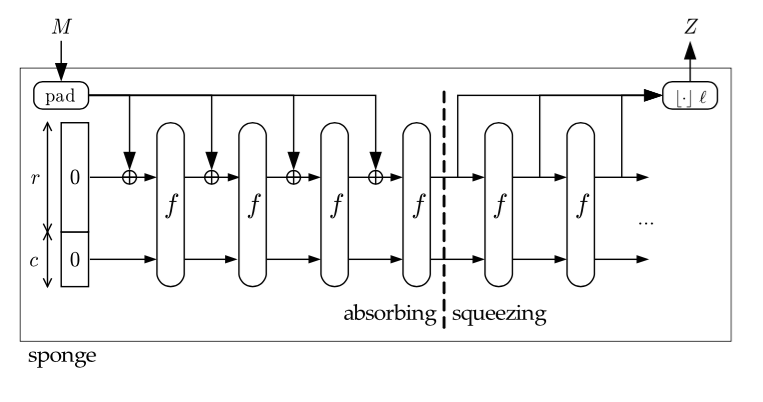
\includegraphics[scale=0.4]{sponge1.png}
\caption{Construction de fonctions en éponge $Z = \textsc{sponge}\lbrack f , pad, r\rbrack (M, l)$}
\end{figure}
  \vfill
\end{frame}

\begin{frame}
  \frametitle{Keccak formellement}
  \vfill
  
    \textbf{Paramètres de la fonction \textsc{Keccak}$\lbrack b, n_r \rbrack$ }:\\
  \begin{itemize}
  \item{ \textbf{$w$}: la longueur fixée des chaines de bits permutés.
  
  \hspace{1cm}$w=2^l$ bits, avec $0 \le l \le 6$.
  }
  \item{ \textbf{$n_r$}: le nombre d'itérations effectuées des routines internes.
  
  \hspace{1cm}$n_r = 12+2\times l$.
  }
  \end{itemize}
  \vspace{1cm}
  \textbf{État de la fonction \textsc{Keccak}}
\begin{itemize}
\item{État constitué de $b = 5 \times 5 \times w$ bits.}
\item{État représenté sous forme matricielle:
\begin{itemize}
\item $5\times w$ lignes indexées horizontalement par x, $0 \le x < 5$.
\item $5 \times w$ colonnes indexées verticalement par y, $0 \le y < 5$.
\item $25$ mots (ou rangées) indexées en profondeur par z, $0 \le z < w$.
\end{itemize}
}
\item{$A\lbrack x,y,z\rbrack$ permet d'accéder à tous les bits de l'état.}
\end{itemize}

  \vfill
\end{frame}

\begin{frame}[fragile]
  \frametitle{État de la fonction Keccak:\\ Représentation matricielle}
  \vfill
  \begin{figure}[H]
    \centering
    \begin{tikzpicture}[scale=0.3]

      \newcommand\faceside[6]{
        \draw (-2+#4,-1+#5) node[]{} node{$\bullet$};
        \pgfmathparse{#1/2+#4}
        \node[text centered, font=\bf] at (\pgfmathresult,-0.7+#5) {#6};
        \foreach \a in {1,...,#1} {
          \foreach \b in {1,...,#2} {
            \fill[fill=white, draw=black] (#4+-1+\a,#5+-1+\b) -- (#4+\a,#5+-1+\b) -- (#4+\a,#5+\b) -- (#4+-1+\a,#5+\b) -- cycle;
          }
          \pgfmathparse{-1+#3}
          \foreach \d [evaluate=\d as \dd using \d*0.5] in {0,...,\pgfmathresult} {
            \fill[fill=white, draw=black] (#4+-1+\a+\d-\dd,#5+#2+\d-\dd) -- (#4+\a+\d-\dd,#5+#2+\d-\dd) -- (#4+\a+\d+0.5-\dd,#5+#2+\d+0.5-\dd) -- (#4+\a+\d-0.5-\dd,#5+#2+\d+0.5-\dd) -- cycle;
          }
        }
        \foreach \c in {1,...,#2} {
          \pgfmathparse{-1+#3}
          \foreach \e [evaluate=\e as \ee using \e*0.5] in {0,...,\pgfmathresult} {
            \fill[fill=white, draw=black] (#4+#1+\e-\ee,#5+-1+\c+\e-\ee) -- (#4+#1+\e+0.5-\ee,#5+-1+\c+\e+0.5-\ee) -- (#4+#1+\e+0.5-\ee,#5+0.5+\c+\e-\ee) -- (#4+#1+\e-\ee,#5+\c+\e-\ee) -- cycle;
          }
        }
      }

      \faceside{1}{1}{1}{-10}{11}{bit}
      \faceside{5}{1}{1}{0}{11}{row}\draw [->, >=latex, dashed] (-2,10) -- (-1,10);\draw (-0.6,10) node[]{$x$};
      \faceside{1}{5}{1}{10}{11}{column}\draw [->, >=latex, dashed] (8,10) -- (8,11);\draw (8,11.4) node[]{$y$};
      \faceside{1}{1}{2}{20}{11}{lane}\draw [->, >=latex, dashed] (18,10) -- (18.8,10.8);\draw (19.1,11.2) node[]{$z$};
      \faceside{5}{1}{2}{-10}{0}{plane}\draw [->, >=latex, dashed] (-12,-1) -- (-11,-1);\draw [->, >=latex, dashed] (-12,-1) -- (-11.1,-0.2);\draw (-10.6,-1) node[]{$x$};\draw (-10.9,0.2) node[]{$z$};
      \faceside{5}{5}{1}{0}{0}{slice}\draw [->, >=latex, dashed] (-2,-1) -- (-1,-1);\draw [->, >=latex, dashed] (-2,-1) -- (-2,0);\draw (-0.6,-1) node[]{$x$};\draw (-2,0.4) node[]{$y$};
      \faceside{1}{5}{2}{10}{0}{sheet}\draw [->, >=latex, dashed] (8,-1) -- (8,0);\draw [->, >=latex, dashed] (8,-1) -- (8.8,-0.2);\draw (8,0.4) node[]{$y$};\draw (9.1,0.2) node[]{$z$};
      \faceside{5}{5}{2}{20}{0}{state}\draw [->, >=latex, dashed] (18,-1) -- (19,-1);\draw [->, >=latex, dashed] (18,-1) -- (18,0);\draw [->, >=latex, dashed] (18,-1) -- (18.8,-0.2);\draw (19.4,-1) node[]{$x$};\draw (18,0.4) node[]{$y$};\draw (19.1,0.2) node[]{$z$};
      
    
    \end{tikzpicture}
    %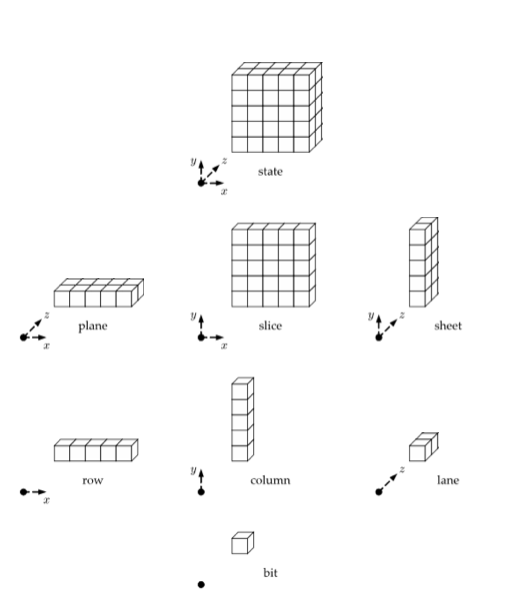
\includegraphics[scale=0.3]{StateArray.png}
    \caption{État manipulé sous forme matricielle A avec $x,y,z \in\llbracket 0,5 \llbracket \times \llbracket 0,5 \llbracket \times \llbracket 0,w \llbracket$}
  \end{figure}
  \vfill
\end{frame}

\begin{frame}
  \frametitle{Une Ronde de \textsc{Keccak}: \textsc{Rnd}}
  \vfill
  \textsc{Keccak}: Pour i de 1 à 24 faire: 
$$\textsc{Rnd}(A,i_r)=\iota ( \chi ( \pi ( \rho (\Theta (A)))), i_r)$$

  \vfill

Les routines d'une ronde \textbf{Rnd}:
  \begin{itemize}
  \item{La routine $\Theta$}
  \item{La routine $\rho$}
  \item{La routine $\pi$}
  \item{La routine $\chi$}
  \item{La routine $\iota$}
   \end{itemize}
  \vfill
\end{frame}


\begin{frame}
  \frametitle{SHA-3}

\vfill
   
\centerline{\textbf{SHA-3 implémente \textsc{Keccak}$\lbrack 1600, 24 \rbrack$}}
 
\bgroup
\def\arraystretch{1.5}
  \begin{table}
\begin{tabular}{l | c | c | c }
$w$ & $l$ & $n_r$ & $b$ \\
\hline
$2^6$ & $6$ & $24$ & $1600 $ 
\end{tabular}
\caption{Paramètres de la fonction \textsc{Keccak} pour SHA-3}

\end{table}

\egroup

\vfill

\textbf{Taille des condensés:}
\begin{itemize}
\item{Fonctions de hachage: 224, 256, 384 et 512 bits}
\item{Fonctions à sortie de taille variable: \textsc{SHAKE128}$(M,l)$ et \textsc{SHAKE128}$(M,l)$  pour une capacité de 256 bits, et une sortie de longueur $l$ }
\end{itemize}
\vspace{1cm}
\vfill
\end{frame}


\begin{frame}<handout:0>
  \frametitle{Plan}
  \tableofcontents[currentsection,subsectionstyle=hide]
\end{frame}

\begin{frame}[fragile]
  \frametitle{Conclusion}

  \begin{minipage}[0.2\textheight]{\textwidth}
    \begin{columns}[T]
      \begin{column}{0.5\textwidth}
        \vspace{2cm}
        \begin{itemize}
        \item{Doutes sur la sécurité de Merkle-Damg\r{a}rd}
          \vspace{1.5cm}
        \item{Apparition de SHA-3, basé sur la construction de l'éponge}
          \vfill
        \end{itemize}
        \vfill
      \end{column}
      \begin{column}{0.5\textwidth}
        
\includegraphics[width=5.5cm]{Conclu-Memoire.jpg}
      \end{column}
      \end{columns}
      \end{minipage}
  \vfill
\end{frame}

\nocite{*}
\bibliographystyle{alpha}

\begin{frame}[allowframebreaks]
  \frametitle{Livres et références}
  \bibliography{biblio}
\end{frame}

%%%%%%%%%%%%%%%%%%%%%%%%%%%%%%%%%%%%%%%%%%%%%%%%%%%%%%%%%%%%%%%%%%%%%%
\begin{frame}
  \vfill
  \centering
  \highlight{\Huge Questions~?}
  \vfill
\end{frame}
